\section{Experiment: Human and LLMs as Labellers}
\label{section:experiment1}

Data labelling, particularly for password strings, is a labour intensive task. To expedite this process, we explored the effectiveness and cost-effectiveness of human versus machine labelling. We recruited freelancers from Fiverr \cite{fiverr2024} to represent the human element. On the machine side, we employed several Large Language Models (LLMs), including GPT-3.5-turbo \cite{gpt3.5}, LLaMA2-13B \cite{llama2}, and 70B, along with the Mistral-7B \cite{mistral7b}. This approach allowed us to compare the precision, efficiency, and financial implications of utilising human labour against AI technologies in the task of labelling complex datasets like passwords.

Several researchers have explored the application of Large Language Models (LLMs) for data labelling \cite{Pangakis_Wolken_Fasching_2023, Liu_2023, Møller_Dalsgaard_Pera_Aiello_2024} with positive results. Notably, this report \cite{refuelllm} cites the accuracy and significant speed up from the language models compared to human labellers.

\subsection{Freelance Labelling}
We tested the utility of freelancers from Fiverr \cite{fiverr2024} for password labelling. We took two samples of 1000 passwords from the \phpbb dataset; we selected passwords that were of length 6 and greater, $L >= 6$, and non-numeric but contained at least one digit. We hired two separate freelancers for \$50 each. The freelancers were proficient in the machine learning data labelling process but were non-native English speakers. They were selected randomly from the responses we received from a posted advert. We would categorise them as non-experts in this domain. We used Google Sheet to share the passwords and monitor the labelling progress. This method proved beneficial as we observed interesting behaviours. We took a hands on approach first by correcting the freelancers at the beginning by checking the first 50 labelled passwords. We had to do a lot of correction.

Interestingly, the second human agent enlisted additional helpers to expedite the labelling process, resulting in errors and inconsistency despite clear instructions. This was evident in the labelling document, where some labellers resorted to copying and pasting from search engine results, prioritising speed over accuracy. In contrast, the first agent focused on accuracy, seeking detailed feedback from us, but exceeded their five-day deadline and showed inconsistency in labelling. Accounting for the hands-on help, the accuracy of the extracted words was $50\% \pm 10\%$; this characteristic was the more accurate compared to chunking, deciphering the structure and tagging the passwords. Ultimately, the output from both agents proved unreliable.



\subsection{Language Models}
\paragraph{Part 1.} We started by fine-tuning the \textbf{GPT-3.5-turbo-0613} model with 825 manually labelled passwords, aiming for JSON-formatted outputs. This fine-tuning was carried out using OpenAI's Python API. The fine-tuning cost was $\sim$\$5 and was completed in a few hours. Testing involved evaluating this model against 300 passwords from the same \phpbb\ distribution, distinct from the training set. This initial fine-tuning, despite using limited data, showed success; however, 41 of the 300 (13.7\%) passwords required relabelling. The model struggled with transformations, especially elongated passwords such as \password{sssssue}, \password{6etter}, and \password{vic20oria}; the latter we assume to be \texttt{"victoria"}. Tokenisation is an important aspect of language models. We believe mislabelling could stem from tokenisation as well. Conducting further tests on the tokenisation method was beyond the scope of this chapter.

Encouraged by promising initial results, we conducted further experiments with additional open-source models. We started with smaller models, LLaMA2-13B and Mistral7B, and fine-tuned them using LoRa~\cite{Hu_Shen_et_al_2021} and QLoRa~\cite{Dettmers_Pagnoni_Holtzman_Zettlemoyer_2023} techniques. The outcomes of the initial experiment, using an 825-labelled training set and a 300-item test set from \phpbb, are presented in Figure~\ref{fig:300comp}.

\begin{figure}[t]
    \centering
    \scalebox{1}{% This file was created with tikzplotlib v0.10.1.
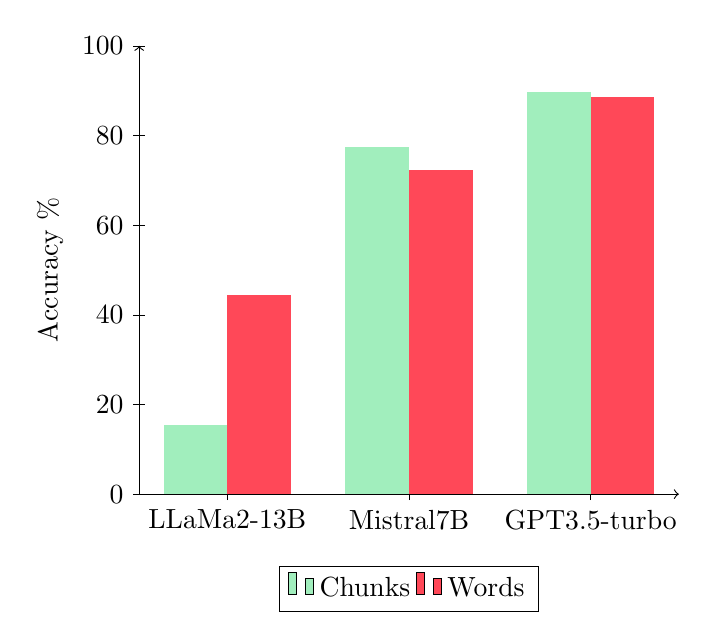
\begin{tikzpicture}

\definecolor{darkgray176}{RGB}{176,176,176}
\definecolor{limegreen018569}{HTML}{FF4858}
\definecolor{teal1293165}{HTML}{A1EEBD}

% \definecolor{xLightGreen}{HTML}{A1EEBD}
% \definecolor{xLightYellow}{HTML}{F6F7C4}
% \definecolor{xLightRed}{HTML}{F6D6D6}
% \definecolor{xLightBlue}{HTML}{7BD3EA}

\begin{axis}[
tick pos=both,
%title={Accuracy of the three models},
x grid style={black},
%xlabel={Model},
legend style={
    at={(0.5, -0.16)}, % Positions the legend below the x-axis
    anchor=north,      % Anchors the legend at its north side (top)
    legend columns=-1  % The number of columns the legend has, -1 for auto
},
xmin=-0.485, xmax=2.485,
xtick style={color=black},
xtick={0,1,2},
xticklabels={LLaMa2-13B,Mistral7B,GPT3.5-turbo},
y grid style={black},
ylabel={Accuracy \%},
ymin=0, ymax=100,
ytick style={color=black},
ytick={0,20,40,60,80,100},
axis lines=left, % This keeps only the left and bottom axis lines
axis line style={->}, % This adds an arrow to the end of the axes
axis y line*=left, % Specifies that the y axis line should be on the left side
axis x line*=bottom, % Specifies that the x axis line should be on the bottom side
]
\draw[draw=none,fill=teal1293165] (axis cs:-0.35,0) rectangle (axis cs:0,15.3333333333333);

\addlegendimage{ybar,ybar legend,draw=none,fill=teal1293165}
\addlegendentry{Chunks}

\draw[draw=none,fill=teal1293165] (axis cs:0.65,0) rectangle (axis cs:1,77.3333333333333);
\draw[draw=none,fill=teal1293165] (axis cs:1.65,0) rectangle (axis cs:2,89.6666666666667);
\draw[draw=none,fill=limegreen018569] (axis cs:2.77555756156289e-17,0) rectangle (axis cs:0.35,44.3333333333333);

\addlegendimage{ybar,ybar legend,draw=none,fill=limegreen018569}
\addlegendentry{Words}

\draw[draw=none,fill=limegreen018569] (axis cs:1,0) rectangle (axis cs:1.35,72.3333333333333);
\draw[draw=none,fill=limegreen018569] (axis cs:2,0) rectangle (axis cs:2.35,88.6666666666667);

\end{axis}

\end{tikzpicture}
}
    \caption{Accuracy of three models in chunking and extracting words from a password string.The models are fine-tuned using 825 passwords from the \phpbb dataset, and are tested on a separate 300 passwords from the same dataset.}
    \label{fig:300comp}
    %\vspace{-1em} 
\end{figure}
%   
\paragraph{Part 2.} In the second phase of our experiment, we augmented our training set by adding 900 passwords from the \hmail dataset. Building on the initial work with GPT-3.5 and Mistral, we expanded our test set to include 3\,062 labelled \hmail passwords. These passwords consisted primarily of characters (without digits) and were not found in dictionaries, indicating they were either phrases or obscure words. We replaced the LLaMa-13B model with a larger LLaMa2 variant, specifically using the \textit{Riiid/sheep-duck-llama-2}\footnote{\url{https://huggingface.co/Riiid/sheep-duck-llama-2-70b-v1.1}} \cite{mukherjee2023orca, platypus2023, Orca-best} model, which benefits from training on a more extensive dataset compared to the standard 70B parameter model.

\begin{figure}[t]
    \centering
    \scalebox{1}{% This file was created with tikzplotlib v0.10.1.
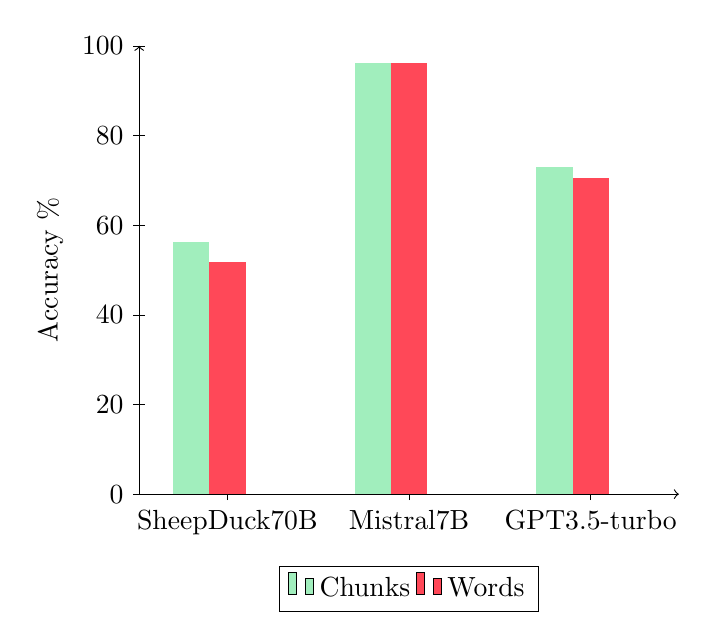
\begin{tikzpicture}

\definecolor{darkgray176}{RGB}{176,176,176}
\definecolor{limegreen018569}{HTML}{FF4858}
\definecolor{teal1293165}{HTML}{A1EEBD}

% \definecolor{xLightGreen}{HTML}{A1EEBD}
% \definecolor{xLightYellow}{HTML}{F6F7C4}
% \definecolor{xLightRed}{HTML}{F6D6D6}
% \definecolor{xLightBlue}{HTML}{7BD3EA}

\begin{axis}[
tick pos=both,
%title={Accuracy of the three models},
x grid style={black},
%xlabel={Model},
legend style={
    at={(0.5, -0.16)}, % Positions the legend below the x-axis
    anchor=north,      % Anchors the legend at its north side (top)
    legend columns=-1  % The number of columns the legend has, -1 for auto
},
xmin=-0.485, xmax=2.485,
xtick style={color=black},
xtick={0,1,2},
xticklabels={SheepDuck70B,Mistral7B,GPT3.5-turbo},
y grid style={black},
ylabel={Accuracy \%},
ymin=0, ymax=100,
ytick style={color=black},
ytick={0,20,40,60,80,100},
axis lines=left, % This keeps only the left and bottom axis lines
axis line style={->}, % This adds an arrow to the end of the axes
axis y line*=left, % Specifies that the y axis line should be on the left side
axis x line*=bottom, % Specifies that the x axis line should be on the bottom side
]
\draw[draw=none,fill=teal1293165] (axis cs:-0.3,0) rectangle (axis cs:-0.1,56.3030698889615);
\addlegendimage{ybar,ybar legend,draw=none,fill=teal1293165}
\addlegendentry{Chunks}

\draw[draw=none,fill=teal1293165] (axis cs:0.7,0) rectangle (axis cs:0.9,96.1463096015676);
\draw[draw=none,fill=teal1293165] (axis cs:1.7,0) rectangle (axis cs:1.9,72.8608752449379);
\draw[draw=none,fill=limegreen018569] (axis cs:-0.1,0) rectangle (axis cs:0.1,51.6982364467668);
\addlegendimage{ybar,ybar legend,draw=none,fill=limegreen018569}
\addlegendentry{Words}

\draw[draw=none,fill=limegreen018569] (axis cs:0.9,0) rectangle (axis cs:1.1,96.1789679947747);
\draw[draw=none,fill=limegreen018569] (axis cs:1.9,0) rectangle (axis cs:2.1,70.4114957544089);
\end{axis}

\end{tikzpicture}
}
    \caption{Chart showing the accuracy of three models in chunking and extracting words from a password string. The models are fine-tuned using 1\,725 manually labelled passwords from the \phpbb and \hmail dataset. Test data is 3062 passwords from the \hmail dataset.}
    \label{fig:shepduckcomp}
    %\vspace{-1em} 
\end{figure}

\subsection{Evaluation}
The models do not generalise well with different structures from ones trained on, e.g. \texttt{rosa38} and \texttt{38rosa} have the reverse grammatical structures. The labelling of the \textit{structure} were predominantly correct except for the digit counts. The models also found reversing the structure difficult. This $A \rightarrow B$ and $B \rightarrow A$ phenomena in LLM is well documented \cite{Berglund_Tong_Kaufmann_Balesni_Stickland_Korbak_Evans_2023}.

The model does not generalise well against languages. We tested the \hmail passwords that contained Spanish words with models that were trained on the \phpbb data and often the models attempted to translate words back into English.

All the models produced well structured JSON data regardless of the amount of data it was fine-tuned with.

Our initial experiment on using language models to label passwords were successful enough to warrant future research in our opinion. Further experimentation of language model is beyond the scope of this chapter and there is significant research avenues to explore. Conducting more experiments with different prompting techniques, synthetic data, more human labelled datasets, and different models can prove beneficial.

